%! TeX program = lualatex

\documentclass{fit-teorsem}

%-------------------------------------------------------------------------------
%                 Fill in seminar information
%-------------------------------------------------------------------------------
\lecturername{Ondřej Kvapil}
\lectureremail{kvapiond@fit.cvut.cz}
\papertitle{Complexity of correspondence $H$-colourings}
\paperauthors{Tomás Feder, Pavol Hell}
\paperlink{https://www.sciencedirect.com/science/article/abs/pii/S0166218X19305128}

%-------------------------------------------------------------------------------
%                 Use custom packages
%-------------------------------------------------------------------------------
\usepackage{enumitem}
\usepackage{amsmath}
\usepackage{amsfonts}
\usepackage{tikz}
\usetikzlibrary{arrows,cd,positioning,shapes,fit}

\tikzset{
	encircle/.style = {draw, circle, inner sep = 0.5mm, color = red},
	dot/.style = {circle, minimum size = 1mm, inner sep = 0mm, draw = black},
	reflexive dot/.style={loop,looseness=17,in=130,out=50},
	reflexive above/.style={->,loop,looseness=7,in=120,out=60},
	reflexive below/.style={->,loop,looseness=7,in=240,out=300},
	reflexive left/.style={->,loop,looseness=7,in=150,out=210},
	reflexive right/.style={->,loop,looseness=7,in=30,out=330}
}

\begin{document}
%-------------------------------------------------------------------------------
%                 Print seminar header
%-------------------------------------------------------------------------------
\maketsheader
%-------------------------------------------------------------------------------
%                 Create your content!
%-------------------------------------------------------------------------------
\thispagestyle{empty}

\section*{Definitions}

\begin{description}
	\item[homomorphism] of a graph $G$ to a graph $H$ is a mapping of the vertex sets $f : V(G) \to V(H)$ 
		that preserves edges, i.e. if $uv$ is an edge of $G$ then $f(u)f(v)$ is an edge of $H$.
	\item[edge-labelled graph] is a graph $G$ together with a mapping (\textit{edge-labelling})
		$\ell : E(G) \to P(H) \times P(H)$, where $P(H)$ denotes the set of all permutations of $V(H)$ 
		and $H$ is a fixed graph (chosen apriori). The label $\ell(xy)$ of an edge $xy$ of $G$ is a pair
		$(\pi, \rho)$ of permutations of $V(H)$, where the permutation $\pi$ is associated with $x$ and
		the permutation $\rho$ with $y$.
	\item[$G$-transversal] of a product $G \times H$ is an induced subgraph $S$ of $G \times H$
		containing exactly one vertex $v_x$ from each set $V_x$ such that the mapping $x \to v_x$
		is an isomorphism of $G$ and $S$. A set $V_x$ is defined as follows:
		$\forall x \in V(G): V_x = \{x\} \times V(H)$.
	\item[correspondence homomorphism] of an edge-labelled graph $G, \ell$ to a graph $H$ is a mapping
		\hbox{$f : V(G) \to V(H)$} such that if $xy \in E(G)$ with $\ell(xy) = (\pi, \rho)$,
		then $\pi(f(x)) \rho(f(y)) \in E(H)$. A correspondence homomorphism of $G, \ell$ to $H$
		will also be called a \textit{correspondence $H$-colouring of $G, \ell$}.

		\begin{center}
		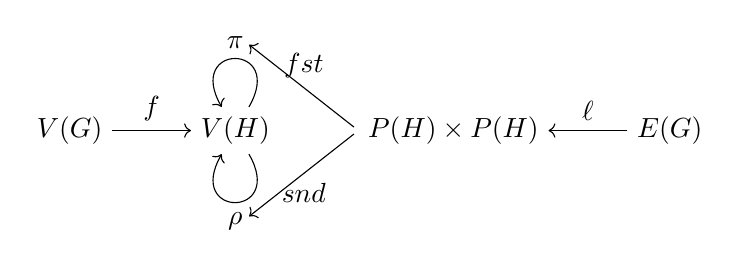
\begin{tikzpicture}
			\node (VG) {$V(G)$};
			\node (VH) [right=of VG] {$V(H)$};
			\draw [->] (VG.east) -- node [above] {$f$} (VH.west);
			\path [->] (VH) edge [reflexive above] node [above] {$\pi$}
				coordinate [xshift = 0.5em, yshift =  0.5em] (pi) (VH);
			\path [->] (VH) edge [reflexive below] node [below] {$\rho$}
				coordinate [xshift = 0.5em, yshift = -0.5em] (rho) (VH);

			\node (PHPH) [right=of VH] {$P(H) \times P(H)$};
			\node (EG) [right=of PHPH] {$E(G)$};
			%\node (EH) [right=of EG] {$E(H)$};
			\draw [->] (EG.west) -- node [above] {$\ell$} (PHPH.east);
			\draw [->, shorten <= 2pt] (PHPH.west) -- node [above] {$fst$} (pi);
			\draw [->, shorten <= 2pt] (PHPH.west) -- node [below] {$snd$} (rho);
		\end{tikzpicture}
		\end{center}

	\item[product of graphs] $G$ and $H$ is the graph $G \times H$ with a vertex set $V(G) \times V(H)$
		where the vertex $(x, u)$ is adjacent to the vertex $(y, v)$ if and only if
		$xy \in E(G) \land uv \in E(H)$. This definition is often referred to as the tensor
		product of graphs or the category-theoretical product of graphs.

		\begin{center}
		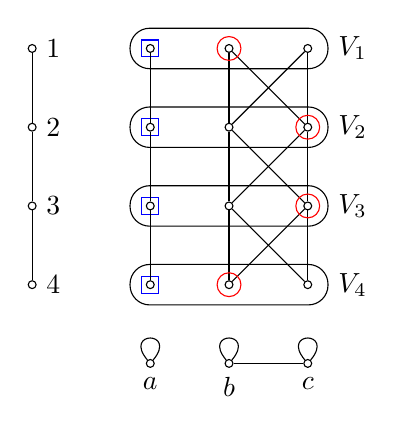
\begin{tikzpicture}
			% without permutations
			\def\gLen{4}
			\foreach\i in {1,...,\gLen}{
				\pgfmathparse{int(\gLen - \i + 1)}
				\let\y\pgfmathresult
				\node [dot]  (\i) at (0.5, \y) [label = right:$\i$] {};
				\node [dot] (a\i) at (2, \y) {};
				\node [dot] (b\i) at (3, \y) {};
				\node [dot] (c\i) at (4, \y) {};

				\node [encircle, rectangle, color = blue, fit = (a\i)] {};

				\node [
					draw, rounded corners = 2.5mm, inner sep = 2mm,
					fit = (a\i) (b\i) (c\i), label = right:$V_\i$
				] (V\i) {};

				\pgfmathparse{int(\i - 1)}
				\let\target\pgfmathresult
				\ifnum\i=1
					% no op
				\else
					\foreach\letter in {a,b,c}{
						\draw (\letter\i.north) -- (\letter\target.south);
					}
					\draw (b\i) -- (c\target);
					\draw (c\i) -- (b\target);
					\draw  (\i.north) --  (\target.south);
				\fi
			}

			\node [encircle, fit = (b1)] {};
			\node [encircle, fit = (c2)] {};
			\node [encircle, fit = (c3)] {};
			\node [encircle, fit = (b4)] {};

			\node [dot] (a) at (2, 0) [label = below:$a$] {};
			\path (a) edge [reflexive dot] (a);
			\node [dot] (b) at (3, 0) [label = below:$b$] {};
			\path (b) edge [reflexive dot] (b);
			\node [dot] (c) at (4, 0) [label = below:$c$] {};
			\path (c) edge [reflexive dot] (c);
			\path (b) edge (c);
		\end{tikzpicture}
		\qquad
		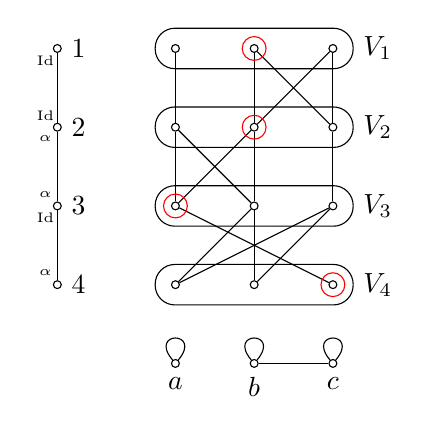
\begin{tikzpicture}
			% permuted
			\def\gLen{4}
			\foreach\i in {1,...,\gLen}{
				\pgfmathparse{int(\gLen - \i + 1)}
				\let\y\pgfmathresult
				\node [dot]  (\i) at (0.5, \y) [label = right:$\i$] {};
				\node [dot] (a\i) at (2, \y) {};
				\node [dot] (b\i) at (3, \y) {};
				\node [dot] (c\i) at (4, \y) {};

				\node [
					draw, rounded corners = 2.5mm, inner sep = 2mm,
					fit = (a\i) (b\i) (c\i), label = right:$V_\i$
				] (V\i) {};

				\pgfmathparse{int(\i - 1)}
				\let\target\pgfmathresult
				\ifnum\i=1
					% no op
				\else
					\ifnum\i=4
						% no op
					\else
						\foreach\letter in {a,b,c}{
							\draw (\letter\i.north) -- (\letter\target.south);
						}
						\draw  (\i.north) --  (\target.south);
					\fi
				\fi
			}

			\draw (4.north) -- (3.south);
			\draw (a2) -- (b3);
			\draw (a3) -- (c4);

			\draw (b1) -- (c2);
			\draw (b2) -- (a3);
			\draw (b3) -- (a4);
			\draw (b3) -- (b4);

			\draw (c1) -- (b2);
			\draw (c3) -- (a4);
			\draw (c3) -- (b4);

			\node [encircle, fit = (b1)] {};
			\node [encircle, fit = (b2)] {};
			\node [encircle, fit = (a3)] {};
			\node [encircle, fit = (c4)] {};

			\node [xshift = -1.5mm, yshift = -1.5mm] (Id1) at (1) {{\tiny Id}};
			\node [xshift = -1.5mm, yshift =  1.5mm] (Id2) at (2) {{\tiny Id}};
			\node [xshift = -1.5mm, yshift = -1.5mm] (alpha2) at (2) {{\tiny $\alpha$}};
			\node [xshift = -1.5mm, yshift =  1.5mm] (alpha3) at (3) {{\tiny $\alpha$}};
			\node [xshift = -1.5mm, yshift = -1.5mm] (Id3) at (3) {{\tiny Id}};
			\node [xshift = -1.5mm, yshift =  1.5mm] (alpha4) at (4) {{\tiny $\alpha$}};

			\node [dot] (a) at (2, 0) [label = below:$a$] {};
			\path (a) edge [reflexive dot] (a);
			\node [dot] (b) at (3, 0) [label = below:$b$] {};
			\path (b) edge [reflexive dot] (b);
			\node [dot] (c) at (4, 0) [label = below:$c$] {};
			\path (c) edge [reflexive dot] (c);
			\path (b) edge (c);
		\end{tikzpicture}
		\end{center}
\end{description}

\section*{Theorems}
\begin{description}
	\item[Theorem 2.1] Suppose $H$ is a reflexive graph.

		If $H$ is a reflexive clique, or a reflexive co-clique, or is isomorphic to a reflexive $K_2 \cup K_2$\footnote{$\cup$ being disjoint union}, then the correspondence $H$-colouring problem is polynomial-time solvable. In all other cases, the correspondence $H$-colouring problem is $NP$-complete.

		If $H$ is a reflexive clique or a reflexive co-clique, then also the correspondence $H$-list-colouring problem is polynomial-time solvable. In all other cases, the correspondence $H$-list-colouring problem is $NP$-complete.

	\item[Theorem 3.1] Suppose $H$ is a reflexive graph.

		If the correspondence $H$-colouring problem is $NP$-complete for graphs $G$ with loops and parallel edges allowed, then it is also $NP$-complete for simple graphs $G$ (without loops or parallel edges).

	\item[Theorem 4.1] Suppose $H$ is a reflexive clique, a reflexive co-clique, or the union of two reflexive $K_2$'s. Then the correspondence $H$-colouring problem is polynomial-time solvable. In the first two cases, the correspondence $H$-list-colouring problem is also polynomial-time solvable.

	\item[Proposition 5.1] The correspondence $(K_1 \cup K_2)$-colouring problem is $NP$-complete.

	\item[Proposition 5.2] The correspondence $(K_1 \cup K_t)$-colouring problem is $NP$-complete,
		$\forall t \ge 2$.

	\item[Proposition 5.3] The correspondence $(K_p \cup K_q \cup K_r \cup \dots \cup K_z)$-colouring
		problem reduces to the correspondence
		$(K_{p + 1} \cup K_{q + 1} \cup K_r \cup \dots \cup K_z)$-colouring problem.

	\item[Proposition 5.4] The correspondence $(K_3 \cup K_3)$-colouring problem is $NP$-complete.

	\item[Proposition 5.5] The correspondence $(K_1 \cup K_1 \cup K_2)$-colouring problem is $NP$-complete.

	\item[Proposition 5.6] The correspondence $H^2$-colouring problem reduces to the correspondence
		$H$-colouring problem.

	\item[Proposition 5.7] If $H$ has diameter two but is not the reflexive path of length two,
		then the correspondence $H$-colouring problem is also $NP$-complete.

	\item[Proposition 5.8] If $H$ is the reflexive path of length two, then the correspondence $H$-colouring
		problem is $NP$-complete.

	\item[Theorem 6.1] Let $H$ be a graph with possible loops. Suppose moreover that if $H$ has both
		a vertex with a loop and a vertex without a loop, then it has no isolated loopless vertices.

		The following cases of the correspondence $H$-colouring problem are polynomial-time solvable.

		\begin{enumerate}
			\item $H$ is a reflexive clique
			\item $H$ is a reflexive co-clique
			\item $H$ is a reflexive $K_2 \cup K_2$
			\item $H$ is an irreflexive $pK_2 \cup qK_1$
			\item $H$ is an irreflexive $K_{2, 2}$
			\item $H$ is a star in which the centre has a loop and the other vertices do not
			\item $H$ is an irreflexive $pK_2$ together with a disjoint reflexive $qK_1$.
		\end{enumerate}

		Otherwise, the correspondence $H$-colouring problem is $NP$-complete. For the correspondence
		$H$-list-colouring problem, the classification is the same, except the cases 3. and 5. are
		$NP$-complete.

	\item[Theorem 6.2] Let $H$ be a graph with possible loops. Suppose moreover that if $H$ has both a vertex
		with a loop and a vertex without a loop, then it has no isolated loopless vertices.

		Then the correspondence $H$-list-colouring problem is polynomial-time solvable in
		cases 1, 2, 4, 6, 7, and is $NP$-complete otherwise.

	\item[Theorem 6.3] Let $H$ be a bipartite graph. Then the by-side correspondence $H$-colouring problem
		is polynomial-time solvable in case 4. above, as well as

		\begin{enumerate}
			\setcounter{enumi}{7}
			\item $H$ is a complete bipartite graph plus any number of isolated vertices,
			\item $H$ is a tree of diameter 3 plus any number of isolated vertices,
			\item $H$ consists of two disjoint copies of $K_{1, 2}$ with white leaves,
				plus any number of black isolated vertices,
			\item $H$ consists of two disjoint copies of $K_{2, 2}$.
		\end{enumerate}

		In all other cases it is $NP$-complete.

	\item[Theorem 6.4] Let $H$ be a bipartite graph. Then the by-side correspondence $H$-list-colouring problem is polynomial-time solvable in cases 4, 8, 9 above, and is $NP$-complete otherwise.
\end{description}

\end{document}
